\documentclass[aspectratio=169]{beamer}
\usepackage{listings}

\beamertemplatenavigationsymbolsempty

\lstset{
  basicstyle=\ttfamily,
}

\title{Schema Inference on Wikidata}
\subtitle{Final presentation}
\author{Lucas Werkmeister}
\date{2019-02-20}

\begin{document}

\frame{\titlepage}

\begin{frame}
  \frametitle{Wikidata}
  \begin{figure}
    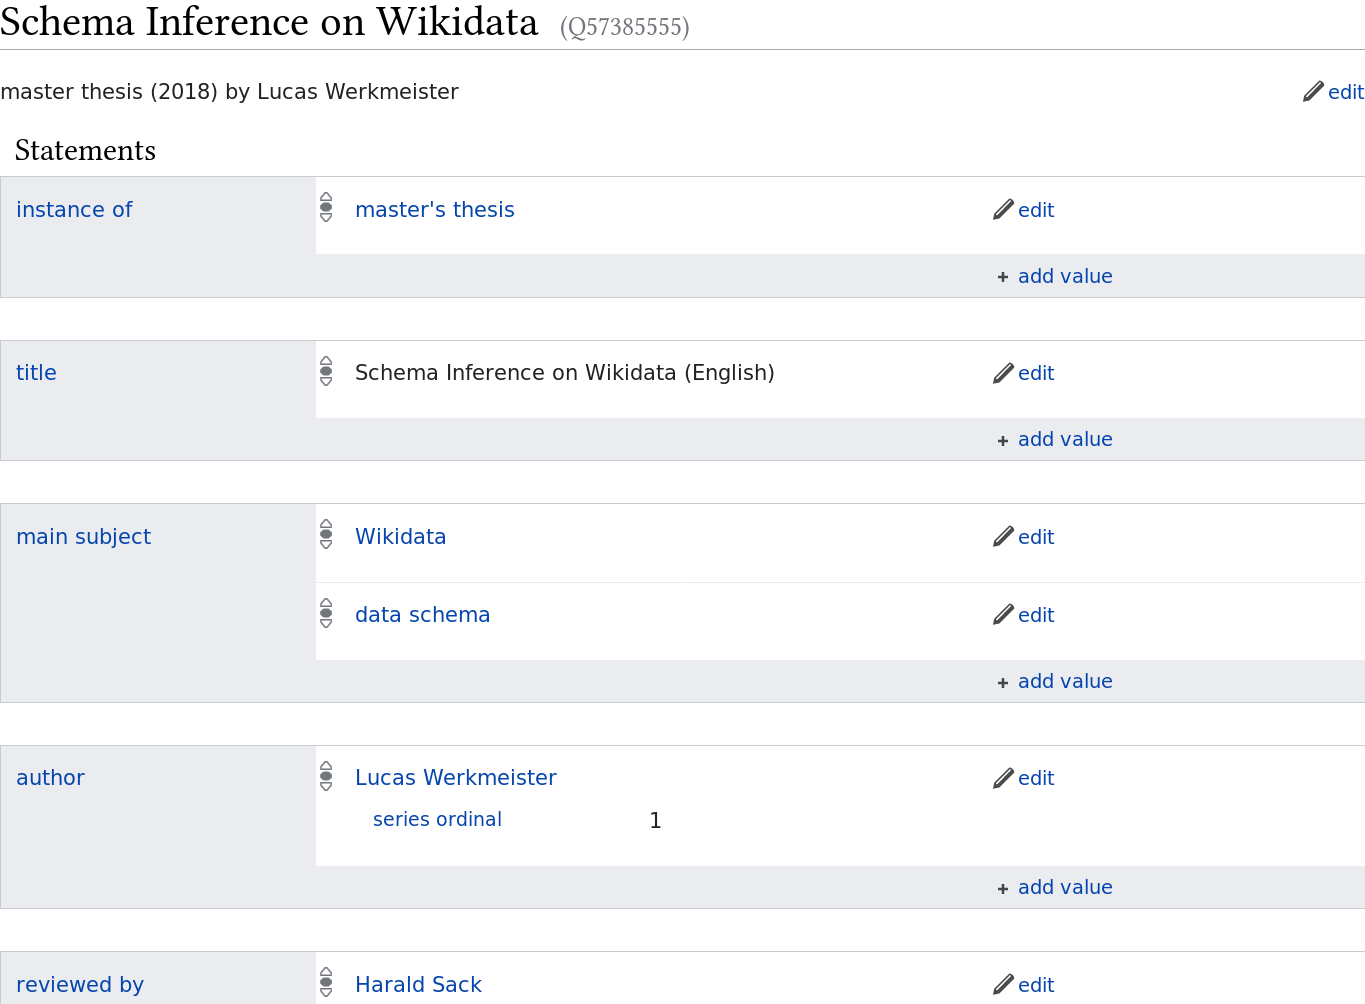
\includegraphics[width=0.7\textwidth]{item}
  \end{figure}
\end{frame}

\begin{frame}
  \frametitle{Wikidata}
  \begin{figure}
    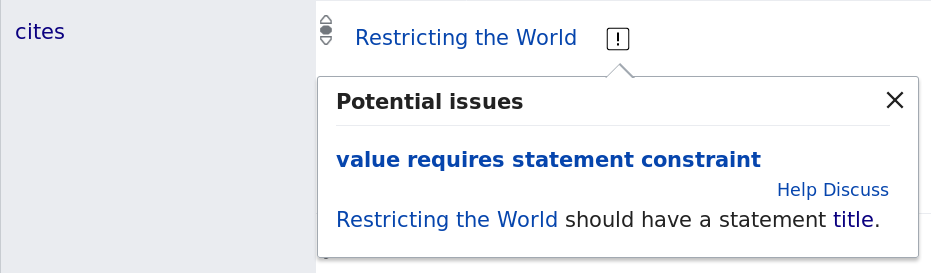
\includegraphics[width=0.8\textwidth]{constraint}
  \end{figure}
\end{frame}

\begin{frame}[fragile]
  \frametitle{RDF}
  \begin{figure}
    \begin{lstlisting}[language=sparql]
wd:Q57385555 rdfs:label "Schema Inference on Wikidata"@en;
  schema:description "master thesis (2018) ..."@en;
  wdt:P31 wd:Q1907875; # instance of: master's thesis
  wdt:P1476 "Schema Inference on Wikidata"@en; # title
  wdt:P50 wd:Q57387675. # author: Lucas Werkmeister

wd:Q57387675 rdfs:label "Lucas Werkmeister"@en;
  wdt:P31 wd:Q5. # instance of: human
    \end{lstlisting}
  \end{figure}
\end{frame}

\begin{frame}[fragile]
  \frametitle{Shape Expressions (ShEx)}
  \begin{figure}
    \begin{lstlisting}[language=sparql]
<master_thesis> {
  wdt:P1476 xsd:langString; # title
  wdt:P50 @<human>+ # author
}

<human> {
  wdt:P569 xsd:dateTime; # date of birth
  wdt:P570 xsd:dateTime? # date of death
}
    \end{lstlisting}
  \end{figure}
\end{frame}

\end{document}
